\documentclass[tikz,border=6pt]{standalone}
\usepackage{amsmath}
\usepackage{xcolor}
\usetikzlibrary{arrows.meta,positioning,calc,fit}

% Conceptual system architecture for assets/diagrams/dynur-architecture.svg.
% Deliberately conceptual: no algorithm names, model sizes or results.
% Build from this directory:
%   pdflatex -interaction=nonstopmode -halt-on-error dynur-architecture.tex
%   pdftocairo -svg dynur-architecture.pdf ../../public/assets/diagrams/dynur-architecture.svg

\definecolor{ink}{HTML}{203746}
\definecolor{muted}{HTML}{647783}
\definecolor{line}{HTML}{AFC2CE}
\definecolor{panel}{HTML}{F8FAFB}
\definecolor{blue1}{HTML}{E6F0F5}
\definecolor{blue2}{HTML}{C9DDE8}
\definecolor{blue3}{HTML}{92B9CD}
\definecolor{blue4}{HTML}{4D86A4}
\definecolor{orange}{HTML}{D77A3B}
\definecolor{orangefill}{HTML}{F6E5D8}

\tikzset{
  >={Stealth[length=2.2mm,width=1.55mm]},
  flow/.style={->, draw=muted, line width=0.85pt},
  dashflow/.style={->, draw=muted, line width=0.75pt, dashed},
  panelbox/.style={draw=line, fill=panel, rounded corners=2.0mm, line width=0.65pt},
  block/.style={draw=line, fill=white, rounded corners=1.2mm, line width=0.65pt, align=center,
    font=\sffamily\small, text=ink, inner sep=2.2mm},
  key/.style={block, draw=blue4, fill=blue1},
  risk/.style={block, draw=orange, fill=orangefill},
  panellabel/.style={font=\sffamily\bfseries\small, text=ink},
  sublabel/.style={font=\sffamily\scriptsize, text=muted, align=center},
}

\begin{document}
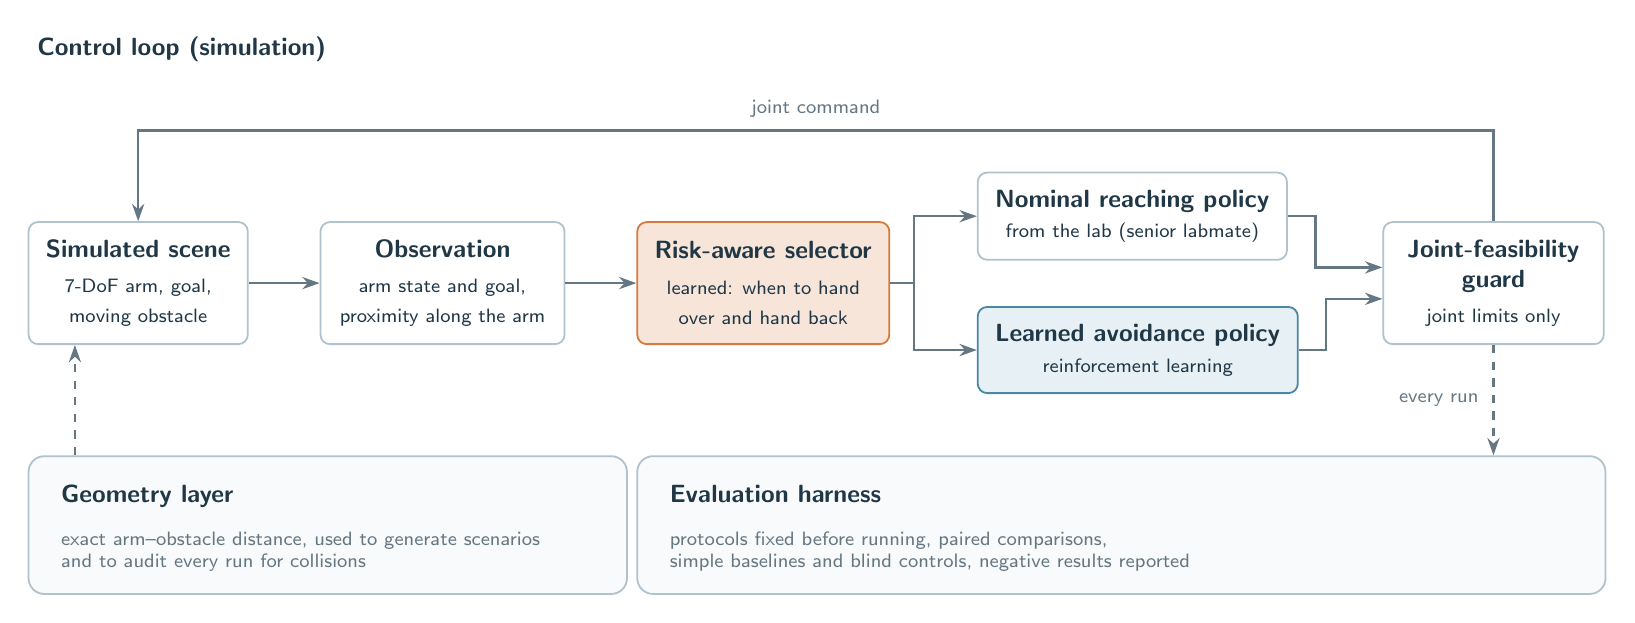
\begin{tikzpicture}[x=1cm,y=1cm]

% Control loop ------------------------------------------------------------------
\node[block, minimum width=2.7cm, minimum height=1.55cm] (scene) at (0,0)
  {\textbf{Simulated scene}\\[0.6mm]{\scriptsize 7-DoF arm, goal,}\\{\scriptsize moving obstacle}};

\node[block, minimum width=3.1cm, minimum height=1.55cm, right=9mm of scene] (obs)
  {\textbf{Observation}\\[0.6mm]{\scriptsize arm state and goal,}\\{\scriptsize proximity along the arm}};

\node[risk, minimum width=2.9cm, minimum height=1.55cm, right=9mm of obs] (sel)
  {\textbf{Risk-aware selector}\\[0.6mm]{\scriptsize learned: when to hand}\\{\scriptsize over and hand back}};

\node[block, minimum width=3.3cm, minimum height=1.05cm, right=11mm of sel, yshift=8.5mm] (reach)
  {\textbf{Nominal reaching policy}\\{\scriptsize from the lab (senior labmate)}};
\node[key, minimum width=3.3cm, minimum height=1.05cm, right=11mm of sel, yshift=-8.5mm] (avoid)
  {\textbf{Learned avoidance policy}\\{\scriptsize reinforcement learning}};

\node[block, minimum width=2.8cm, minimum height=1.55cm, anchor=west] (guard)
  at ([xshift=12mm]reach.east |- sel.east)
  {\textbf{Joint-feasibility}\\\textbf{guard}\\[0.6mm]{\scriptsize joint limits only}};

\draw[flow] (scene) -- (obs);
\draw[flow] (obs) -- (sel);
\draw[flow] (sel.east) -- ++(3mm,0) |- (reach.west);
\draw[flow] (sel.east) -- ++(3mm,0) |- (avoid.west);
\draw[flow] (reach.east) -- ++(3.5mm,0) |- ([yshift=2mm]guard.west);
\draw[flow] (avoid.east) -- ++(3.5mm,0) |- ([yshift=-2mm]guard.west);

% Joint command back into the scene.
\draw[flow] (guard.north) -- ++(0,1.15) -| node[sublabel, pos=0.25, above=0.4mm] {joint command} (scene.north);

\node[panellabel, anchor=south west] at ([yshift=19mm]scene.north west) {Control loop (simulation)};

% Offline tooling ---------------------------------------------------------------
\node[panelbox, minimum width=7.6cm, minimum height=1.75cm, anchor=north west] (geom)
  at ([yshift=-14mm]scene.south west) {};
\node[panellabel, anchor=north west] at ([xshift=3mm,yshift=-2.5mm]geom.north west) {Geometry layer};
\node[sublabel, anchor=north west, align=left] at ([xshift=3mm,yshift=-8.5mm]geom.north west)
  {exact arm--obstacle distance, used to generate scenarios\\and to audit every run for collisions};

\path let \p1 = (sel.west), \p2 = (guard.east) in
  node[panelbox, minimum width=\x2-\x1, minimum height=1.75cm, anchor=north west] (eval)
  at ([yshift=-14mm]sel.south west) {};
\node[panellabel, anchor=north west] at ([xshift=3mm,yshift=-2.5mm]eval.north west) {Evaluation harness};
\node[sublabel, anchor=north west, align=left] at ([xshift=3mm,yshift=-8.5mm]eval.north west)
  {protocols fixed before running, paired comparisons,\\simple baselines and blind controls, negative results reported};

\draw[dashflow] ([xshift=6mm]geom.north west) -- ([xshift=6mm]scene.south west);
\draw[dashflow] (guard.south) -- node[sublabel, left=0.6mm] {every run} (guard.south |- eval.north);

\end{tikzpicture}
\end{document}
